\chapter{TINJAUAN PUSTAKA}

\section{Koefisien Restitusi}

\subsection{Definisi dan Konsep Dasar}
Koefisien restitusi ($e$) adalah parameter dasar dalam mekanika yang digunakan untuk mengukur tingkat keelastisan tumbukan antara dua benda. Konsep ini pertama kali dikemukakan oleh Sir Isaac Newton melalui hukum restitusi Newton (\textit{Newton's law of restitution}). Hukum tersebut menyatakan bahwa perbandingan kecepatan pemisahan sesudah tumbukan dengan kecepatan pendekatan sebelum tumbukan merupakan konstanta untuk material tertentu \citep{goldsmith1999theory}.

Dalam konteks fisika, koefisien restitusi memberikan gambaran mengenai seberapa besar energi kinetik yang dapat dipulihkan setelah terjadinya tumbukan. Nilai ini sangat berguna dalam berbagai aplikasi teknik, mulai dari desain \textit{bola olahraga} hingga analisis \textit{kecelakaan kendaraan}.

\subsection{Formulasi Matematis}
Secara matematis, koefisien restitusi dapat didefinisikan sebagai hubungan antara kecepatan relatif sebelum dan sesudah tumbukan terjadi. Gambar \ref{fig:teori-figure-1} memperlihatkan diagram skematik yang menggambarkan komponen kecepatan sebelum dan sesudah tumbukan \textit{bola} dengan permukaan datar.

\begin{figure}
    \centering
    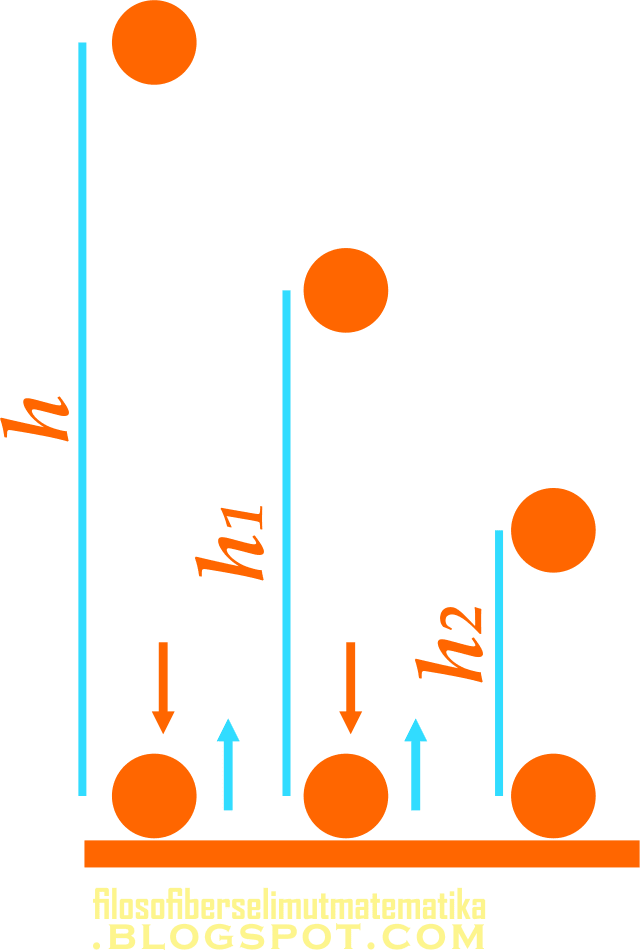
\includegraphics[width=0.3\linewidth]{images/gambar restitusi.png}
    \caption{Diagram skematik tumbukan \textit{bola} dengan permukaan datar menunjukkan komponen kecepatan sebelum dan setelah tumbukan}
    \label{fig:teori-figure-1}
\end{figure}

\begin{equation}
    e = \frac{|v_{r}'|}{|v_{r}|} = \frac{|v_2' - v_1'|}{|v_1 - v_2|}
\end{equation}

dengan:
\begin{itemize}
    \item $e$ = koefisien restitusi (tanpa dimensi)
    \item $v_{r}'$ = kecepatan relatif sesudah tumbukan (m/s)
    \item $v_{r}$ = kecepatan relatif sebelum tumbukan (m/s)
    \item $v_1', v_2'$ = kecepatan benda 1 dan 2 sesudah tumbukan (m/s)
    \item $v_1, v_2$ = kecepatan benda 1 dan 2 sebelum tumbukan (m/s)
\end{itemize}

Untuk kasus khusus tumbukan vertikal dengan permukaan datar, perhitungan koefisien restitusi dapat disederhanakan. Dalam hal ini, analisis menjadi lebih mudah karena dapat menggunakan hubungan antara ketinggian awal dan ketinggian pantulan:

\begin{equation}
    e = \sqrt{\frac{h_2}{h_1}}
\end{equation}

dengan:
\begin{itemize}
    \item $h_1$ = tinggi awal pelepasan benda (m)
    \item $h_2$ = tinggi pantulan maksimum sesudah tumbukan (m)
\end{itemize}

\subsection{Klasifikasi Tumbukan Berdasarkan Nilai Koefisien Restitusi}
Berdasarkan nilai koefisien restitusi yang diperoleh, tumbukan dapat dikelompokkan menjadi tiga kategori utama. Setiap kategori mencerminkan karakteristik energi yang berbeda-beda.

Tumbukan \textit{elastis sempurna} terjadi apabila nilai koefisien restitusi sama dengan satu ($e = 1$). Pada kondisi ini, seluruh energi kinetik sistem tetap terjaga. Fenomena semacam ini biasanya dijumpai pada tumbukan antar\textit{partikel} dalam kondisi ideal \citep{stronge2018impact}. 

Kondisi berikutnya adalah tumbukan \textit{tidak elastis sempurna} yang memiliki nilai koefisien restitusi nol ($e = 0$). Dalam keadaan ini, seluruh energi kinetik relatif berubah menjadi energi internal seperti panas dan deformasi permanen \citep{johnson1987contact}. 

Kategori terakhir merupakan tumbukan \textit{tidak elastis sebagian} dengan rentang nilai antara nol dan satu ($0 < e < 1$). Pada kondisi ini, sebagian energi kinetik hilang dalam proses tumbukan. Kondisi seperti ini merupakan fenomena yang umum dijumpai dalam tumbukan nyata \citep{cross2002coefficient}.

\subsection{Hubungan Koefisien Restitusi dengan Sifat Material dan Deformasi}
Nilai koefisien restitusi sangat bergantung pada karakteristik intrinsik material. Karakteristik tersebut meliputi \textit{modulus elastisitas} ($E$), \textit{batas luluh} (\(\sigma_y\)), dan sifat \textit{viskoelastik} material \citep{meyer2020coefficient}. 

Material yang memiliki \textit{modulus elastisitas} tinggi seperti baja atau keramik umumnya menunjukkan nilai $e$ yang lebih besar. Hal ini berbeda dengan material yang memiliki \textit{modulus} rendah seperti polimer atau busa \citep{brancazio1981physics}. 

Proses deformasi selama tumbukan berlangsung dapat dibagi menjadi dua fase yang saling berkaitan, yaitu \textit{kompresi} dan \textit{restorasi}. Pada fase \textit{kompresi}, energi kinetik diubah menjadi energi deformasi elastis dan plastis. Sementara itu, pada fase \textit{restorasi}, energi deformasi elastis dikembalikan menjadi energi kinetik. Adapun energi deformasi plastis menjadi energi disipasi \citep{hartono2019analisis}.

\subsection{Faktor-Faktor yang Memengaruhi Koefisien Restitusi}

Beberapa faktor memengaruhi nilai koefisien restitusi dalam proses tumbukan nyata. \textit{Kecepatan tumbukan} merupakan faktor pertama yang cukup signifikan. Peningkatan \textit{kecepatan tumbukan} menyebabkan deformasi plastis yang lebih besar sehingga menurunkan nilai $e$ \citep{smith2018experimental}. 

Karakteristik permukaan juga berperan penting dalam menentukan nilai koefisien restitusi. \textit{Kekasaran permukaan} ($R_a$) dan kondisi pelumasan memengaruhi energi disipasi melalui gesekan \citep{penner2002physics}. 

\textit{Temperatur lingkungan} memberikan pengaruh terhadap sifat material. Peningkatan \textit{temperatur} menurunkan \textit{modulus elastisitas} material yang berdampak pada penurunan nilai $e$ \citep{lamb1945hydrodynamics}. 

\textit{Geometri benda} turut memengaruhi distribusi tegangan selama tumbukan berlangsung. Bentuk dan ukuran relatif benda menentukan pola deformasi yang terjadi \citep{stronge2018impact}.

\section{Sensor Ultrasonik HC-SR04}

\subsection{Prinsip Kerja dan Teori Dasar}
Sensor ultrasonik HC-SR04 bekerja berdasarkan prinsip \textit{time-of-flight} (TOF) dengan menggunakan gelombang ultrasonik berfrekuensi 40 kHz \citep{fauzi2020pengujian}. Prinsip kerja sensor ini mengikuti persamaan dasar yang menghubungkan jarak dengan waktu tempuh gelombang:

\begin{equation}
    d = \frac{v \cdot t}{2}
\end{equation}

dengan:
\begin{itemize}
    \item $d$ = jarak objek dari sensor (m)
    \item $v$ = kecepatan suara dalam udara (m/s)
    \item $t$ = waktu tempuh gelombang ultrasonik (s)
    \item Faktor 2 dalam penyebut disebabkan oleh perjalanan gelombang \textit{bolak-balik}
\end{itemize}

Kecepatan suara dalam udara dapat dihitung dengan menggunakan persamaan yang mempertimbangkan pengaruh \textit{temperatur lingkungan}:

\begin{equation}
    v = 331,4 + 0,6 \cdot T
\end{equation}

dengan:
\begin{itemize}
    \item $T$ = \textit{temperatur udara} dalam Celsius (°C)
    \item 331,4 = kecepatan suara pada 0°C (m/s)
    \item 0,6 = \textit{koefisien temperatur} (m/s·°C)
\end{itemize}

\subsection{Spesifikasi Teknis}
Sensor HC-SR04 memiliki karakteristik teknis yang mendukung aplikasi pengukuran jarak dengan presisi tinggi \citep{siregar2021sensor}. Sensor ini beroperasi pada tegangan 5V DC dengan konsumsi arus sebesar 15 mA. Rentang pengukurannya mencapai 2 cm hingga 400 cm dengan akurasi ±3 mm. 

Sudut deteksi sensor mencapai 15° yang memungkinkan deteksi objek dalam area yang cukup luas. Sensor menggunakan frekuensi ultrasonik 40 kHz untuk transmisi gelombang. Untuk mengaktifkan proses pengukuran, sensor memerlukan durasi pulsa \textit{trigger} minimum 10 $\mu$s.

\subsection{Konfigurasi Pin dan Antarmuka}
Sensor HC-SR04 dirancang dengan empat pin utama. Setiap pin memiliki fungsi spesifik dalam sistem pengukuran. Pin VCC berfungsi sebagai input tegangan 5V DC untuk suplai daya sensor. Pin GND merupakan \textit{ground} atau referensi tegangan 0V. Pin \textit{Trig} adalah input untuk memicu pengiriman gelombang ultrasonik. Pin \textit{ECHO} adalah output yang memberikan pulsa dengan lebar yang sebanding dengan jarak objek yang dideteksi. 

Konfigurasi pin ini ditunjukkan pada Gambar \ref{fig:teori-figure-2} yang menggambarkan diagram pin dan konfigurasi sensor ultrasonik HC-SR04.

\begin{figure}
    \centering
    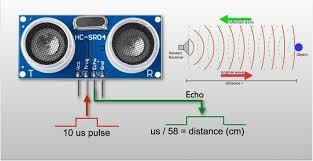
\includegraphics[width=0.5\linewidth]{images/hcsr.jpg}
    \caption{Diagram pin dan konfigurasi sensor ultrasonik HC-SR04}
    \label{fig:teori-figure-2}
\end{figure}

\subsection{Algoritma Pengukuran}
Proses pengukuran jarak menggunakan sensor HC-SR04 mengikuti algoritma yang terstruktur dan dapat diandalkan \citep{rohman2021aplikasi}. Proses dimulai dengan memberikan pulsa HIGH selama 10 $\mu$s pada pin \textit{Trigger} untuk mengaktifkan transmisi gelombang ultrasonik. 

Selanjutnya, pin \textit{ECHO} akan berubah menjadi HIGH ketika gelombang ultrasonik dipancarkan. Pin ini kembali menjadi LOW ketika gelombang pantul diterima oleh sensor. Sistem kemudian mengukur durasi pulsa HIGH pada pin \textit{ECHO} dan menghitung jarak menggunakan persamaan TOF yang telah ditetapkan. Algoritma ini memastikan pengukuran yang konsisten dan akurat dalam berbagai kondisi operasional.

\section{Mikrokontroler ESP8266}

\subsection{Arsitektur dan Spesifikasi}
ESP8266 adalah \textit{System-on-Chip} (SoC) yang mengintegrasikan mikrokontroler 32-bit berbasis arsitektur \textit{Tensilica L106} dengan modul \textit{Wi-Fi IEEE 802.11 b/g/n} \citep{rodrigues2018vision}. Sistem ini menggunakan prosesor \textit{Tensilica L106 32-bit RISC} dengan \textit{clock} hingga 160 MHz yang memberikan performa komputasi yang memadai untuk aplikasi \textit{IoT}. 

Konfigurasi memori meliputi 64 KB RAM instruksi dan 96 KB RAM data untuk operasi waktu nyata. Sistem dilengkapi \textit{flash} eksternal berkapasitas 512 KB hingga 4 MB untuk penyimpanan program dan data. 

Sistem dilengkapi dengan 16 pin digital I/O yang dapat dikonfigurasi sesuai kebutuhan aplikasi. Terdapat satu kanal \textit{ADC 10-bit} dengan rentang 0-1V untuk pembacaan sensor analog. \textit{Interface komunikasi} yang tersedia meliputi \textit{UART}, \textit{SPI}, dan \textit{I2C}. Mikrokontroler beroperasi pada tegangan 3,3V dengan konsumsi daya 80 mA dalam mode aktif dan 20 $\mu$A dalam mode \textit{deep sleep} untuk efisiensi energi.

\begin{figure}
    \centering
    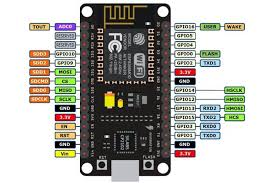
\includegraphics[width=0.5\linewidth]{images/esp 8266.jpg}
    \caption{Modul ESP8266 dengan konfigurasi pin GPIO}
    \label{fig:teori-figure-3}
\end{figure}

\subsection{Konfigurasi Pin dan Fungsionalitas}
Konfigurasi pin ESP8266 dirancang untuk fleksibilitas maksimum dalam berbagai aplikasi \textit{IoT}. Pin GPIO0 hingga GPIO16 berfungsi sebagai I/O digital dengan kemampuan \textit{PWM} dan \textit{interrupt}. Hal ini memungkinkan \textit{interfacing} dengan berbagai sensor dan aktuator. 

Pin \textit{ADC} khusus disediakan untuk pembacaan sensor analog yang memerlukan konversi sinyal analog ke digital. Pin \textit{TX/RX} digunakan untuk komunikasi \textit{UART} yang memfasilitasi \textit{serial debugging} dan komunikasi dengan perangkat eksternal. 

Pin \textit{RST} berfungsi sebagai \textit{reset} untuk \textit{restart} sistem dalam kondisi tertentu. Adapun pin \textit{EN} merupakan \textit{enable pin} untuk aktivasi chip secara keseluruhan. Gambar \ref{fig:teori-figure-3} menunjukkan modul ESP8266 dengan konfigurasi pin GPIO yang lengkap.

\subsection{Pemrograman dan Development Environment}
ESP8266 mendukung berbagai lingkungan pengembangan yang memfasilitasi implementasi aplikasi \textit{IoT} dengan fleksibilitas tinggi. \textit{Arduino IDE} dengan \textit{ESP8266 Core} merupakan platform yang paling populer. Platform ini memungkinkan penggunaan sintaks \textit{Arduino} untuk pemrograman yang familiar bagi sebagian besar \textit{developer} \citep{monk2016programming}. 

\textit{Framework} alternatif yang didukung meliputi \textit{ESP-IDF} untuk pengembangan tingkat lanjut, \textit{MicroPython} untuk \textit{rapid prototyping}, dan \textit{NodeMCU Lua} untuk pengembangan berbasis \textit{scripting}. Keberagaman platform ini memungkinkan \textit{developer} memilih lingkungan yang paling sesuai dengan kebutuhan proyek dan tingkat kompleksitas aplikasi.

\section{\textit{Internet of Things} (IoT)}

\subsection{Definisi dan Konsep Fundamental}
\textit{Internet of Things} (IoT) adalah paradigma komputasi yang memungkinkan objek fisik (\textit{things}) terhubung ke \textit{internet} dan saling berkomunikasi untuk bertukar data secara otomatis tanpa intervensi manusia \citep{ashton2009internet}. Konsep ini melibatkan integrasi sensor, aktuator, komunikasi nirkabel, dan sistem komputasi \textit{awan} untuk menciptakan ekosistem digital yang cerdas \citep{ray2018survey}. 

Implementasi \textit{IoT} memungkinkan pengumpulan data waktu nyata dari lingkungan fisik. Selain itu, \textit{IoT} juga memungkinkan pemrosesan data menggunakan algoritma cerdas dan respons otomatis terhadap kondisi tertentu.

\subsection{Arsitektur IoT}
Arsitektur \textit{IoT} umumnya terdiri atas empat lapisan utama yang saling terintegrasi untuk menciptakan sistem yang komprehensif \citep{weber2010governance}. 

Lapisan \textit{persepsi} merupakan fondasi sistem yang terdiri atas sensor dan aktuator. Lapisan ini mengumpulkan data lingkungan dan melakukan aksi berdasarkan instruksi yang diterima. 

Lapisan \textit{jaringan} menangani transmisi data melalui berbagai protokol komunikasi seperti \textit{Wi-Fi}, \textit{Bluetooth}, \textit{ZigBee}, atau \textit{LoRaWAN} sesuai dengan kebutuhan aplikasi. 

Lapisan \textit{pemrosesan} melakukan analisis dan pemrosesan data menggunakan algoritma yang sesuai, baik secara lokal maupun di \textit{cloud computing}. 

Lapisan \textit{aplikasi} menyediakan antarmuka pengguna dan layanan aplikasi yang memungkinkan interaksi antara pengguna dengan sistem \textit{IoT}.

\subsection{Protokol Komunikasi IoT}
Sistem \textit{IoT} menggunakan berbagai protokol komunikasi yang dipilih berdasarkan kebutuhan spesifik aplikasi. Pemilihan protokol didasarkan pada jangkauan, konsumsi daya, dan \textit{throughput} data. 

\textit{Wi-Fi IEEE 802.11} digunakan untuk komunikasi lokal berkecepatan tinggi dengan konsumsi daya yang relatif tinggi namun memberikan \textit{bandwidth} yang luas. 

\textit{Bluetooth} dan \textit{Bluetooth Low Energy} (BLE) cocok untuk komunikasi jarak pendek dengan konsumsi daya rendah. Protokol ini ideal untuk aplikasi \textit{wearable} dan sensor personal. 

\textit{ZigBee} berdasarkan \textit{IEEE 802.15.4} dirancang khusus untuk jaringan sensor nirkabel dengan topologi \textit{mesh} yang dapat mengcover area yang luas. 

\textit{LoRaWAN} (\textit{Long Range Wide Area Network}) dikembangkan untuk komunikasi jarak jauh dengan daya rendah. Protokol ini sangat sesuai untuk aplikasi \textit{smart city} dan \textit{monitoring lingkungan}.

\subsection{Message Queuing Telemetry Transport (MQTT)}
\textit{MQTT} adalah protokol komunikasi \textit{publish-subscribe} yang dirancang khusus untuk aplikasi \textit{IoT} dengan \textit{bandwidth} terbatas dan koneksi tidak stabil \citep{zhang2021iot}. Protokol ini beroperasi di atas \textit{TCP/IP} dan menggunakan arsitektur \textit{broker-client} yang memungkinkan komunikasi yang efisien dan dapat diandalkan. 

Desain \textit{MQTT} memprioritaskan efisiensi \textit{bandwidth} dan ketahanan terhadap gangguan jaringan. Hal ini menjadikannya ideal untuk aplikasi \textit{IoT} yang memerlukan transmisi data waktu nyata dengan konsumsi daya minimal.

\subsubsection{Arsitektur MQTT}
Sistem \textit{MQTT} terdiri atas tiga komponen utama yang bekerja secara sinergis. \textit{Publisher} merupakan perangkat yang mengirim data ke \textit{broker} dengan \textit{topik} tertentu yang telah ditentukan. 

\textit{Broker} berfungsi sebagai \textit{server} yang menerima, memfilter, dan mendistribusikan pesan kepada \textit{subscriber} yang berlangganan \textit{topik} tertentu. 

\textit{Subscriber} adalah perangkat yang menerima data dari \textit{broker} berdasarkan \textit{topik} yang telah mereka \textit{subscribe} sebelumnya. Arsitektur ini memungkinkan komunikasi \textit{many-to-many} yang efisien dan fleksibel.

\subsubsection{Quality of Service (QoS) dalam MQTT}
\textit{MQTT} mendefinisikan tiga level \textit{Quality of Service} (QoS) untuk pengiriman pesan. Hal ini memberikan fleksibilitas dalam menentukan tingkat keandalan transmisi data \citep{anderson2019digital}. 

QoS 0 atau \textit{At most once} memungkinkan pesan dikirim maksimal satu kali tanpa konfirmasi. Tingkat ini cocok untuk data yang tidak kritis dan dapat mentolerir kehilangan data. 

QoS 1 atau \textit{At least once} menjamin pesan terkirim minimal satu kali dengan kemungkinan duplikasi. Tingkat ini sesuai untuk data penting yang memerlukan konfirmasi penerimaan. 

QoS 2 atau \textit{Exactly once} menjamin pesan terkirim tepat satu kali tanpa duplikasi. Tingkat ini ideal untuk data kritis yang memerlukan integritas tinggi.

\subsubsection{Struktur Topik MQTT}
\textit{Topik MQTT} menggunakan struktur hierarkis dengan separator "/" 
untuk mengorganisir data secara sistematis dan logis. Contoh implementasi 
dalam penelitian ini menggunakan struktur seperti berikut
\begin{verbatim}
sensor/koefisien_restitusi/bola_tenis/tinggi_awal
sensor/koefisien_restitusi/bola_tenis/tinggi_pantul
\end{verbatim}
Struktur ini memungkinkan kategorisasi data berdasarkan jenis sensor, parameter yang 
diukur, objek pengukuran, dan jenis data spesifik.



\section{Karakteristik Material Bola}

\subsection{Klasifikasi Material Berdasarkan Sifat Mekanik}
Material bola dapat diklasifikasikan berdasarkan sifat mekaniknya yang memengaruhi koefisien restitusi secara signifikan \citep{kalnins2018separation}. 

Material \textit{elastis} seperti polimer dengan \textit{modulus elastisitas} tinggi menunjukkan kemampuan pemulihan bentuk yang baik setelah deformasi. Hal ini menghasilkan koefisien restitusi yang relatif tinggi. 

Material \textit{viskoelastis} termasuk karet alam dan sintetis memiliki karakteristik yang menggabungkan sifat elastis dan viskos. Pada material ini, respons terhadap beban bergantung pada waktu dan kecepatan pembebanan. 

Material \textit{komposit} yang merupakan kombinasi serat dan matriks polimer menunjukkan sifat mekanik yang dapat disesuaikan. Penyesuaian dilakukan berdasarkan orientasi serat dan jenis matriks yang digunakan.

\subsection{Hubungan Modulus Elastisitas dengan Koefisien Restitusi}
\textit{Modulus elastisitas} ($E$) material didefinisikan sebagai perbandingan antara \textit{tegangan normal} ($\sigma$) terhadap \textit{regangan normal} ($\varepsilon$). Nilai ini memberikan ukuran kekakuan material:

\begin{equation}
    E = \frac{\sigma}{\varepsilon}
\end{equation}

dengan:
\begin{itemize}
    \item $E$ = \textit{modulus elastisitas} (Pa)
    \item $\sigma$ = \textit{tegangan normal} (Pa)
    \item $\varepsilon$ = \textit{regangan normal} (tanpa dimensi)
\end{itemize}

\textit{Tegangan} dan \textit{regangan} dapat dihitung menggunakan persamaan yang menghubungkan gaya dan deformasi dengan sifat geometris material:

\begin{equation}
    \sigma = \frac{F}{A}
\end{equation}

\begin{equation}
    \varepsilon = \frac{\Delta L}{L_0}
\end{equation}

dengan:
\begin{itemize}
    \item $F$ = gaya yang diterapkan (N)
    \item $A$ = luas penampang ($m^2$)
    \item $\Delta L$ = perubahan panjang (m)
    \item $L_0$ = panjang awal (m)
\end{itemize}

\subsection{Geometri Bola dan Kalkulasi Volume}
\textit{Geometri bola} memainkan peran penting dalam analisis karakteristik material dan perhitungan parameter fisik. \textit{Volume bola} ($V$) dihitung menggunakan persamaan geometris fundamental:

\begin{equation}
    V = \frac{4}{3}\pi r^3
\end{equation}

dengan:
\begin{itemize}
    \item $V$ = \textit{volume bola} (m³)
    \item $r$ = \textit{jari-jari bola} (m)
    \item $\pi$ = konstanta pi (3,14159...)
\end{itemize}

\textit{Luas permukaan bola} ($A$) diberikan oleh persamaan yang menentukan area kontak potensial selama tumbukan:

\begin{equation}
    A = 4\pi r^2
\end{equation}

dengan:
\begin{itemize}
    \item $A$ = \textit{luas permukaan bola} ($m^2$)
\end{itemize}

\subsection{Material Bola dalam Penelitian}
Penelitian ini menggunakan lima jenis bola dengan karakteristik material yang berbeda. Hal ini bertujuan memberikan variasi yang komprehensif dalam analisis koefisien restitusi \citep{avancini2020physical}. 

\textit{Bola tenis meja} terbuat dari \textit{selulosa asetat} dengan densitas rendah yang memberikan karakteristik pantulan yang responsif dan konsisten. 

\textit{Bola bekel} menggunakan \textit{karet sintetis} dengan elastisitas tinggi yang memungkinkan pemulihan energi yang efisien selama proses tumbukan. 

\textit{Bola plastik} terbuat dari \textit{polietilena} dengan sifat termoplastik yang menunjukkan deformasi plastis yang signifikan selama tumbukan. 

\textit{Bola karet} menggunakan \textit{karet alam} dengan sifat viskoelastis yang memberikan respons yang bergantung pada kecepatan deformasi. 

\textit{Bola baseball} menggunakan material \textit{komposit berlapis} yang menggabungkan berbagai material untuk mengoptimalkan performa dan durabilitas. 

Setiap material memiliki karakteristik unik yang memengaruhi respons dinamis selama proses tumbukan. Hal ini tercermin dalam nilai koefisien restitusi yang berbeda untuk setiap jenis bola dan memberikan wawasan mendalam tentang hubungan antara sifat material dan perilaku tumbukan.